\documentclass{article}
\usepackage{graphicx}
\usepackage{geometry}
\geometry{a4paper, margin=1in}

\title{Wing Optimization Report}
\date{2025-06-08}

\begin{document}

\maketitle

\section{Executive Summary}
This report details the optimization of a wing design with a fixed area of 400 m$^2$ and a span of 60 m, targeting a lift coefficient (CL) of 0.5. The optimization aimed to minimize drag by adjusting taper, dihedral, twist, and sweep. The drag coefficient converged to approximately 0.010805206. While the optimization process appears successful, certain aspects of the final design suggest potential areas for further refinement. The optimization converged in 18 iterations using the SLSQP optimizer.

\section{Problem Formulation}
The optimization problem was formulated as follows:
\begin{itemize}
    \item Objective Function: Minimize drag
    \item Trim Condition: CL = 0.5
    \item Geometric Constraints: Wing area (S) = 400 m$^2$, Span (b) = 60 m
    \item Design Variables: Taper, Dihedral, Twist, Sweep
\end{itemize}

\section{Analysis of Results}

\subsection{Wing Geometry and Aerodynamic Performance}
The final wing shape exhibits a low dihedral angle, a linear twist distribution, and a nearly elliptical lift distribution, as expected for drag minimization. However, deviations from a perfect ellipse suggest room for improvement.

\begin{figure}[h!]
    \centering
    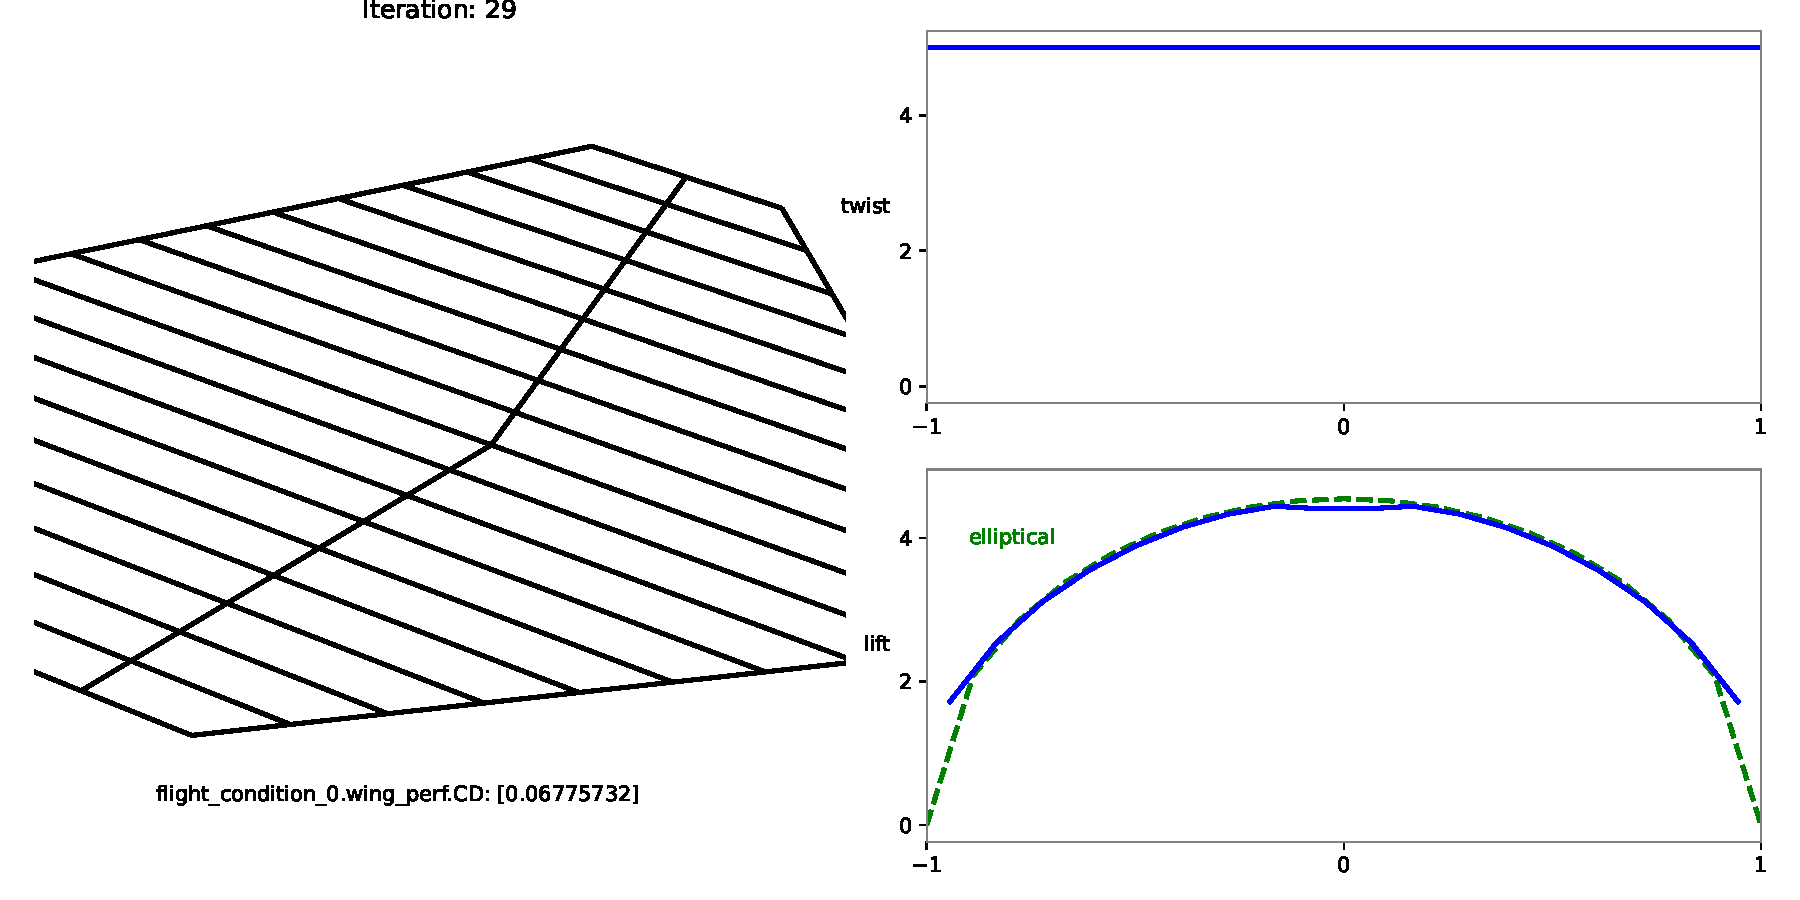
\includegraphics[width=0.7\textwidth]{./Optimized_Wing.pdf}
    \caption{Optimized Wing Visualization}
    \label{fig:optimized_wing}
\end{figure}
Figure \ref{fig:optimized_wing} visualizes the optimized wing.  The linear twist is apparent in the figure, as well as the final optimized shape.

\subsection{Optimization Performance}
The optimization converged quickly using the SLSQP optimizer, indicating that the optimizer may be appropriate for the design problem. However, if the design space is made more complex, or if other constraints are added, then the number of iterations may need to be increased.

\section{Recommendations}

\subsection{Explore Dihedral}
The dihedral angle is pinned at a low value. Consider either removing the design variable or broadening its bounds to investigate if a non-zero dihedral can further reduce induced drag. Ensure sufficient panels are used to resolve winglets if they are present, and consider optimizing winglet geometry.

\subsection{Refine Twist Distribution}
The linear twist distribution suggests a need for a more complex design space. Increase the number of control points for twist to allow for a more optimal distribution.

\subsection{Explore Taper Ratio}
Experiment with different taper ratios, as a well-chosen taper ratio can significantly improve span efficiency and better approximate an elliptical lift distribution.

\subsection{Further Optimize Sweep}
Ensure the sweep angle is physically reasonable for the aircraft's intended speed regime. Since it's a subsonic aircraft, sweep is expected to be low.

\subsection{Investigate Constraints}
Check for any active constraints that may be preventing further drag reduction. Relaxing constraints, if possible, could lead to a better optimum. The optimization converged near the bounds of some design variables; explore expanding those bounds if physically reasonable. Add a manufacturability constraint.

\subsection{Aerodynamic Center Verification}
Verify that the final wing configuration's aerodynamic center is within an acceptable range for stability purposes.

\section{Additional Considerations}

\subsection{Manufacturability}
The optimized wing geometry should be assessed for manufacturability. Sharp changes in twist, dihedral, or sweep can increase manufacturing costs.

\subsection{VLM Limitations}
OpenAeroStruct uses a Vortex Lattice Method (VLM) for aerodynamic analysis, which has limitations in accurately capturing viscous effects, stall behavior, and complex flow phenomena. For a more detailed analysis, consider using a higher-fidelity CFD solver after initial optimization with OpenAeroStruct.

\subsection{Reynolds Number}
Ensure the Reynolds number used in the analysis is representative of the actual flight conditions. Since OpenAeroStruct is VLM, profile drag may be inaccurate due to viscous effects not being modeled properly.

\end{document}